\documentclass[12pt, a4paper, twoside]{article}
\usepackage{fancyhdr}
\pagestyle{fancy}
%\fancyhf{}
\renewcommand{\headrulewidth}{0pt}
\addtolength{\headwidth}{\marginparsep}
\addtolength{\headwidth}{\marginparwidth}
\rhead[]{\large\textbf{EXD}}
\usepackage{fontspec}
\setmainfont{Times New Roman}
\usepackage[margin=2.5cm]{geometry}
\usepackage{amsmath,amsfonts,amsthm}
\usepackage{graphicx}
% \graphicspath{{../pdfbox/}}
%% bibliography setting nature style, footnotesize in bibliography and
%% avoiding in in articles
\usepackage[style=nature,defernumbers=true,maxnames=1,firstinits=true,uniquename=init,backend=bibtex8,arxiv=abs,mcite]{biblatex}
\usepackage{jabbrv}
\DeclareFieldInputHandler{journaltitle}{%
  \def\NewValue{\JournalTitle{#1}}}
\bibliography{../biblio}
%\renewcommand{\bibfont}{\normalfont\footnotesize}
\renewbibmacro{in:}{%
  \ifentrytype{article}{}{%
  \printtext{\bibstring{in}\intitlepunct}}}
\DeclareFieldFormat[article]{title}{}
\AtBeginBibliography{\footnotesize}
%% to set line space in bibliography
\usepackage{setspace}
%% to add affiliation to the title
\usepackage[affil-it]{authblk}
\renewcommand\Affilfont{\itshape\small}
\setlength{\affilsep}{.2em}
%% for figure caption
\usepackage[format=plain, font=scriptsize,labelfont=bf]{caption}
%% for figure wrapping
\usepackage{wrapfig}
%% for reference in a multi col
\usepackage{multicol}
\captionsetup[figure]{font={footnotesize, stretch=1.}, belowskip=.01pt,
  aboveskip=0.3pt}
%\captionsetup[figure]{font={footnotesize, stretch=1.}, skip=0pt}
%% titling
\makeatletter
\renewcommand{\maketitle}{\bgroup\setlength{\parindent}{0pt}
\begin{flushleft}
{\LARGE
  \textbf{\@title}}

\vspace{0.3ex}

  \@author
\end{flushleft}\egroup
}
\makeatother
\title{SOL profile and fluctuations in different divertor recycling conditions in H-Mode plasmas}
\author{N. Vianello$^{1}$,
  N. Walkden$^{2}$,
  M. Dunne$^{3}$,
  B. Lomanowski$^{4}$,
  E. Wolfrum$^3$,
  C. Tsui$^{5, 6}$,
  M. Griener$^3$,
  B. Tal$^3$,
  D. Refy$^7$,
  D Brida$^3$,
  I. Cziegler$^8$,
  O. F{\'e}vrier$^5$,
  H. De Oliveira$^{5}$,
  M. Agostini$^{1}$,
  S. Aleiferis$^9$,
  M. Bernert$^3$,
  J. Boedo${^6}$,
  M. Brix$^{2}$,
  D. Carralero$^{10}$,
  I. Carvalho$^{2, 15}$,
  L. Frassinetti$^{11}$,
  C. Giroud$^2$,
  A. Hakola$^{12}$,
  A. Huber$^{13}$,
  J. Karhunen$^{14}$,
  A. Karpushov$^{5}$,
  B. Labit$^5$,
  A. Meigs$^2$,
  V. Naulin$^{15}$,
  T. Pereira$^{16}$,
  H. Reimerdes$^5$,
  C. Theiler$^5$,
  the ASDEX-Upgrade Team,
  the TCV-Team,
  the EUROfusion MST1 Team$^{*}$
  and JET Contributors$^{**}$}

\affil{
  $^1$Consorzio RFX, Padova,Italy,
  $^{2}$CCFE, Culham, UK,
  $^{3}$Max-Planck-Institut f{\"u}r Plasmaphysik, Garching, Germany,
  $^{4}$Oak Ridge National Laboratory,
  $^{5}$EPFL-SPC, Switzerland,
  $^6$UCSD,  La Jolla, USA,
  $^7$Wigner Research Centre for Physics,
  $^{8}$York Plasma Institute, University of York, UK,
  $^9$NCSR Athens GR,
  $^{10}$CIEMAT Laboratorio Nacional de Fusi{\'o}n, Madrid, Spain,
  $^{11}$Division of Fusion Plasma Physics, KTH, Stockholm SE,
  $^{12}$VTT, Espoo, Finland,
  $^{13}$Forschungszentrum Julich,
  $^{14}$Aalto University, Espoo, Finland,
  $^{15}$DTU,  Copenhagen, Denmark,
  $^{16}$IST/IPFN, Lisbon, Portugal
  $^{*}$See the author list B. Labit et al 2019 Nucl. Fusion 59 086020,
$^{**}$See the authors list E. Joffrin et al 2019 Nucl. Fusion 59 112021}
%%% ------------------------------------------------------------
%%% BEGIN DOCUMENT
%%% ------------------------------------------------------------
\begin{document}
\maketitle
%
\vspace{-1.2em}
% {\it \small Corresponding Author:} {nicola.vianello@igi.cnr.it}

Plasma Exhaust and Plasma Wall Interaction are subjects of intense studies
in the context of fusion energy research for the understanding of the amount of heat
loads and the lifetime of different Plasma Facing
Components. In order to ensure reliable
predictive edge modeling in this context, it is mandatory to
determine the transport properties of the Scrape Off Layer (SOL), a
region which is largely influenced by the presence of turbulent
filaments which contribute to particle and energy losses in both L and
H mode. From the ITER divertor perspective, to
keep the power fluxes acceptable for target material,
high neutral pressure and partial detachment are needed to
ensure maximum tolerable loads \cite{pitts:2019}.
\begin{wrapfigure}[12]{l}{100mm}
%\begin{figure}[!t]
%\centering
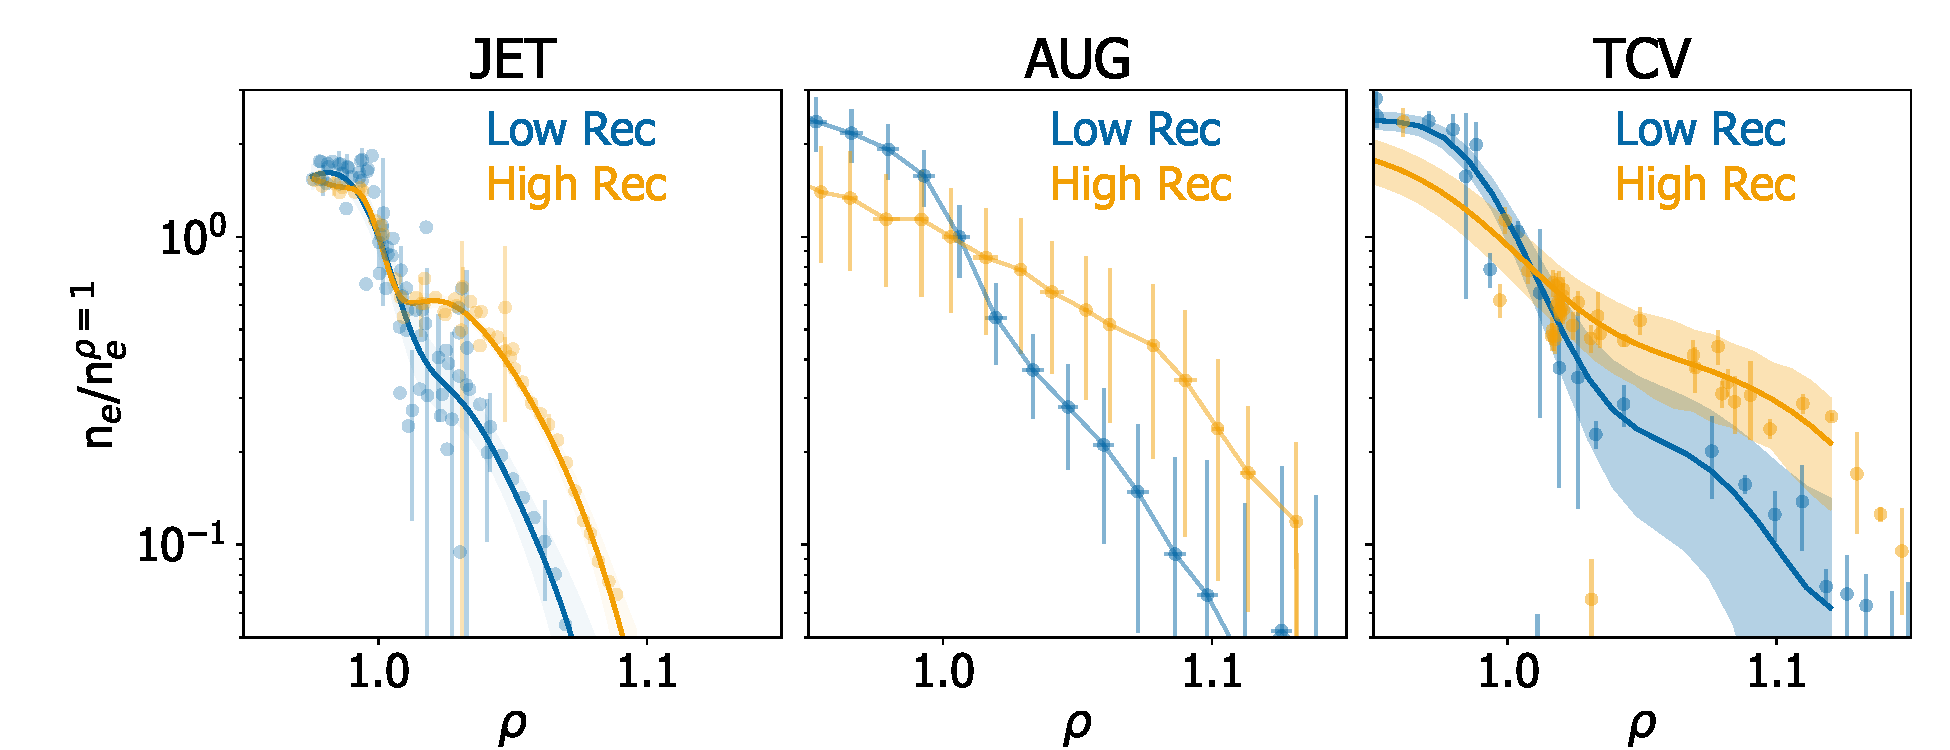
\includegraphics[width=100mm]{../pdfbox/AllUpstreamProfiles_synopsis.pdf}
\caption{Upstream profiles, normalized with
  respect to values at the separatrix in different recycling
  conditions for JET (a),  AUG (b) and TCV (c). In all the cases symbols represent raw data whereas the solid line represent a
 Gaussian Process Regression fit}
%\vspace{-2.6ex}
\label{fig:figProfile}
\end{wrapfigure}
Thus experimental investigation
of SOL transport needs to be extended to these regimes.
In present experiments the regimes matching the ITER divertor operational point are obtained
with high gas throughput leading to high density. In L-Mode
these operational conditions are associated with the appearance of a
\emph{density shoulder}
i.e. progressive flattening of the density
scrape off layer profile at high density
\cite{Asakura:1997is,LaBombard:2001ks,
  Carralero:2017gb}. It has been shown that density shoulder appear
starting from high-recycling regimes and become broader after target
density rollover \cite{vianello:nf2019}, even
though differences have been observed depending on divertor geometry
\cite{Wynn:2018gp}, or if high recycling conditions are achieved
through impurity seeding rather than high fuelling
\cite{Wynn:2018gp,Kuang:2019248}.
The density shoulder is actually accompained by
an increase of the filamentary activity
\cite{Carralero:2017gb,vianello:nf2019,Kuang:2019248}, together with an increase of
their associated heat and particle convective transport \cite{Carralero:2017gb}.
Preliminary investigations suggested that similar inter-ELM SOL
density profile broadening is observed in H-mode as well
\cite{Muller:2015jt,Carralero:2017gb,vianello:nf2019}, with a stronger
dependence on the neutral pressure \cite{vianello:nf2019}. The
possible increase of convective heat and particle fluxes to the wall
poses serious issues in terms of acceptable sputtering yield of the
first wall. In H-mode,
in case of highly dissipative divertor with high gas throughput, the
plasma changes its stability properties moving towards a small-ELM
regime \cite{Harrer:2018jn} where a clear increase of
the SOL density decay length is observed.
Despite the
large effort, a comprehensive understanding
of the mechanism leading to an H-mode shoulder formation is presently
lacking and this motivated a joint experimental program within the
Eurofusion framework.
The present contribution will show an unique comparison of H-Mode SOL
density shoulder properties across 3 different devices, JET, ASDEX-Upgrade (AUG) and
TCV focusing on the SOL profile evolution in different divertor recycling
states, correlating the observed profile modification with different turbulent SOL
plasma transport.
\begin{wrapfigure}[12]{l}{100mm}
%\begin{figure}[!t]
%\centering
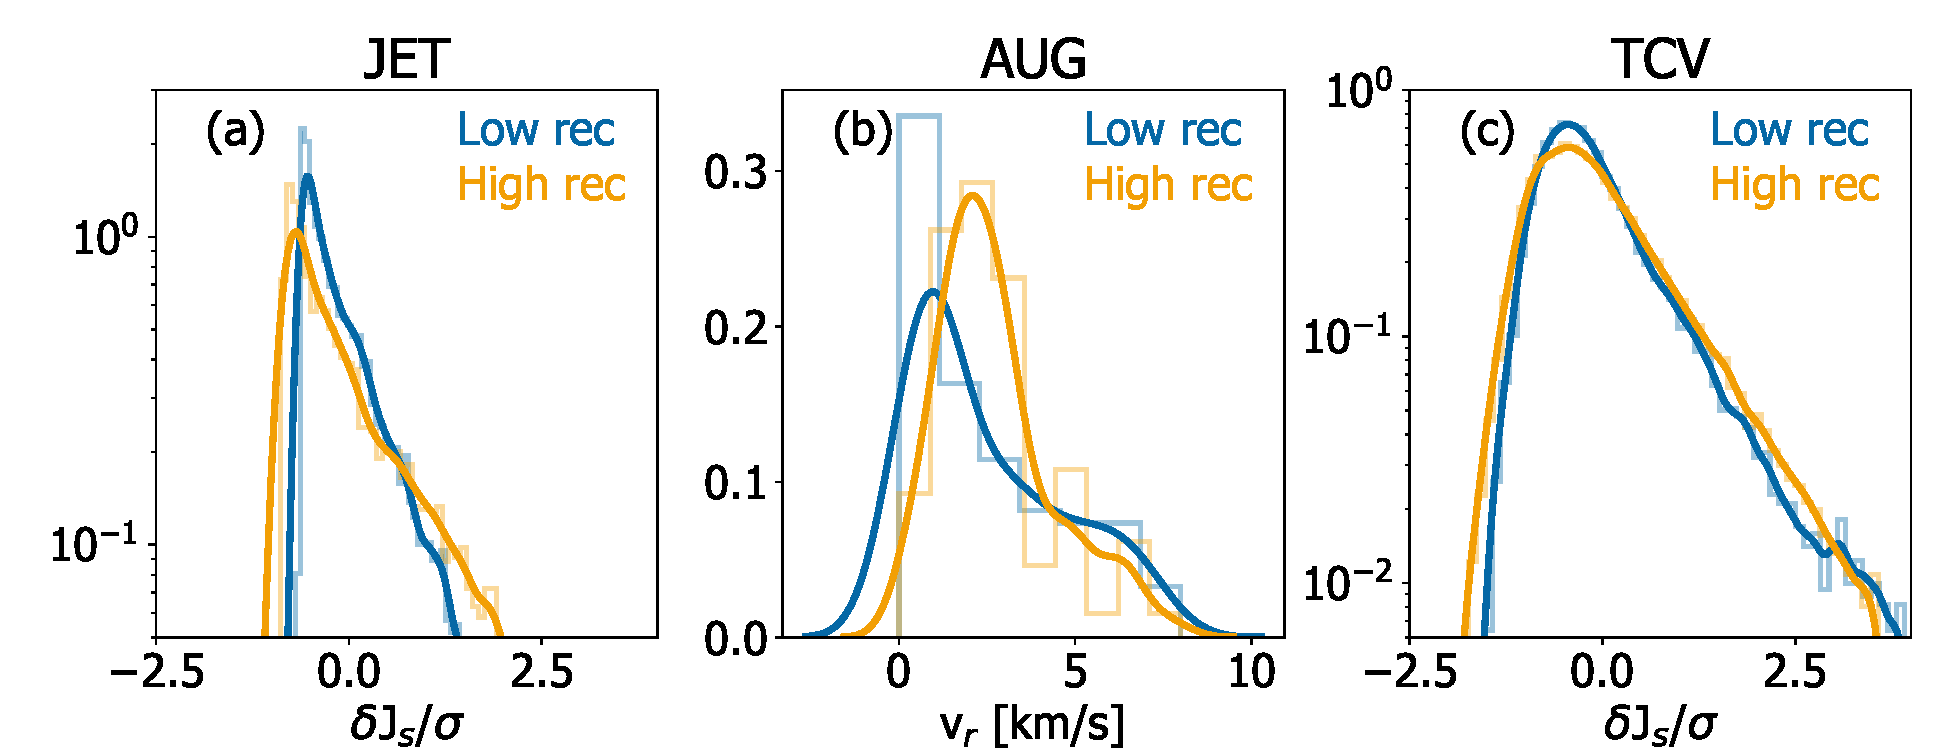
\includegraphics[width=100mm]{../pdfbox/SynopsisFluctuationCombined.pdf}
\caption{Fluctuation properties in different recycling states for the
  3 devices:(a) PDF of Jsat fluctuations at the wall on JET (b)
  inter-ELM filament velocity in the far SOL from THB diagnostic (c) PDF of Jsat fluctuations at the wall on TCV}
\vspace{-2.6ex}
\label{fig:figFluctuations}
\end{wrapfigure}

On JET, 2MA/2.3T low $\delta$ plasma with 16 MW of
applied NBI power were analyzed, with different levels of fueling exploring different divertor shapes
in order to tackle the dependence of neutral compression as well
\cite{Tamain:2015cx}.
On AUG 0.8MA/2.5T scenarios at different power levels (from 3 to 17 MW) and different fuelling
schemes were analyzed in order to explore a wide range of divertor
parameters and recycling states.
Finally on TCV high-$\delta$ low current (0.18 MA)
discharges were investigated with an additional 1 MW of NBI heating
with different fueling levels and locations. In all the devices we have been able to
identify conditions where inter-ELM density profiles at different recycling states exhibit a clear profile broadening as shown in
figure \ref{fig:figProfile}. In order to access the contribution of SOL
turbulence induced convective transport in modifying the SOL profile,
fluctuations in the main SOL and at the wall have been investigated
using different diagnostics in the various machines as shown in
\ref{fig:figFluctuations}. On AUG,  filaments velocities of
inter-ELM filaments have been determined using the Thermal Helium Beam
diagnostic \cite{Griener:20183cf} and compared with the fluctuations
observed in high-recycling state during the small-ELM regime. The
comparison of the Probability Distribution Function (PDF) of these velocities is shown in
\ref{fig:figFluctuations} (b) and a clear increase of the filament velocity
during high recycling state is observed. For TCV and JET we show the
PDF of the ion saturation current
density J$_s$ as measured at the wall by mean of embedded langmuir
probes respectively in panels (a) and (c) of figure
\ref{fig:figFluctuations}.
In high density/high recycling state more skewed PDFs are
observed for both the machines suggesting an increase of the
fluctuation induced convective transport towards the first wall.
These experimental results form an excellent basis to benchmark SOL
modelling under various conditions in differently sized machines,
providing a more complete characterization of the
explored conditions in terms of divertor properties, upstream
profiles, SOL fluctuation and induced transport and pedestal evolution. These observations
consequently will strongly contribute to improve
the understanding of SOL transport in conditions relevant fo the ITER divertor operation.

\begingroup
\setstretch{0.8}
{\footnotesize\textbf{Acknowledgment}\\
This work has been carried out within the framework of the EUROfusion Consortium and has received funding from the Euratom research and training programme 2014 - 2018 and 2019 - 2020 under grant agreement No 633053. The views and opinions expressed herein do not necessarily reflect those of the European Commission.}
\begin{multicols}{2}
\setlength\bibitemsep{0pt}
\printbibliography[heading=none]
\end{multicols}
\endgroup

\end{document}

% \begin{wrapfigure}[10]{l}{100mm}
% \centering
% 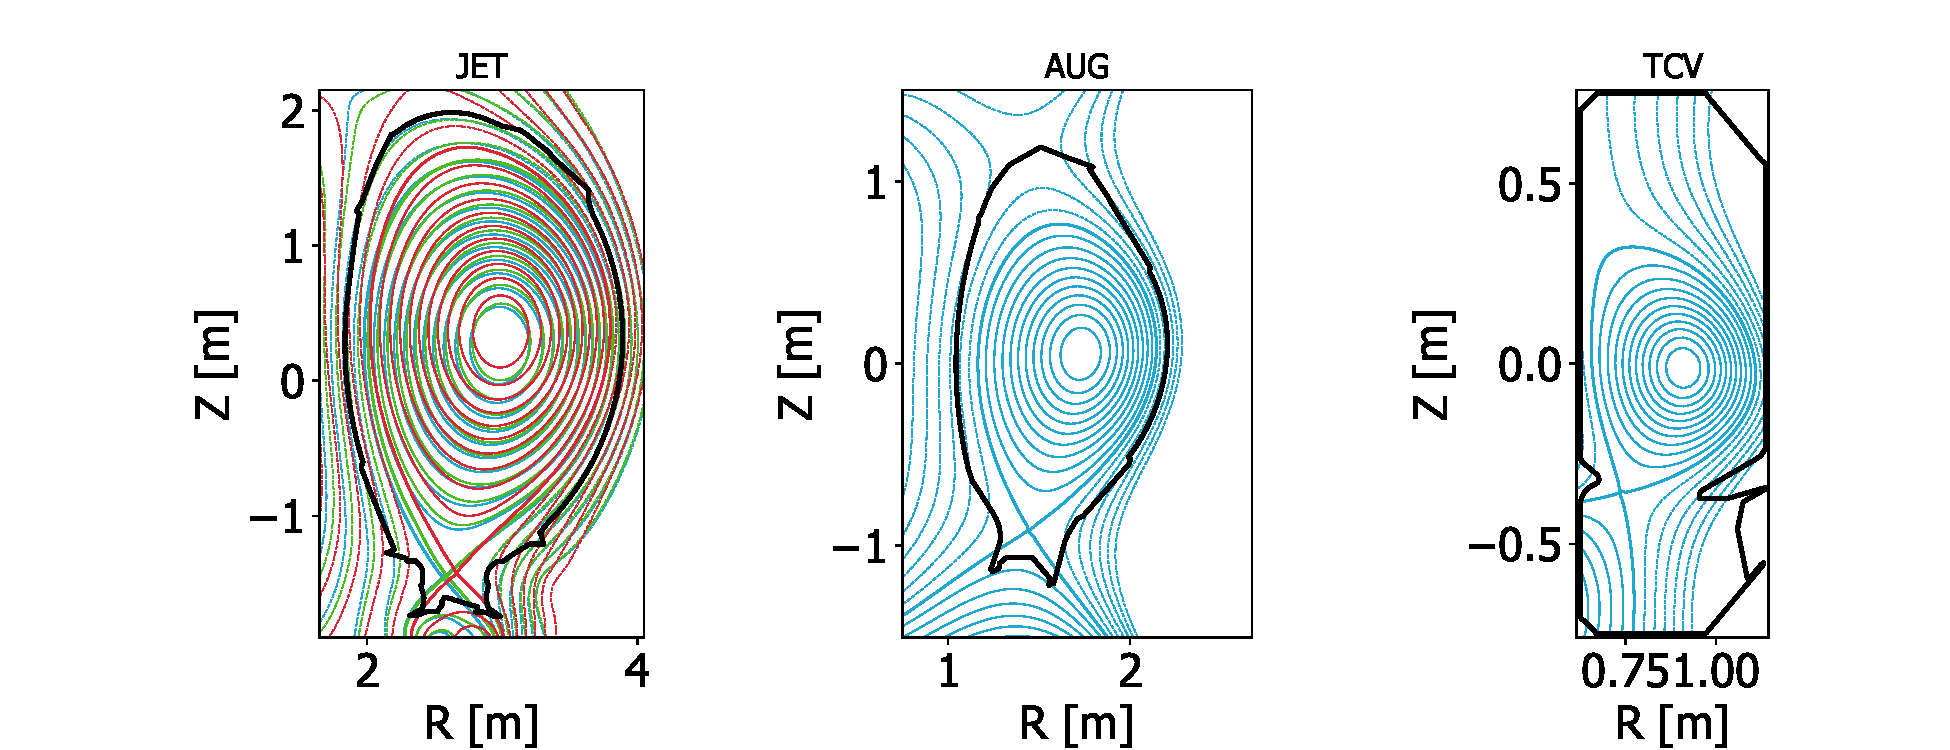
\includegraphics[width=100mm]{../pdfbox/AllEquilibria.pdf}
% \caption{Plasma shapes investigated in all the three devices. For JET
%   the 3 different configuration are shown as well}
% \vspace{-2.6ex}
% \label{fig:figEquilibria}
% \end{wrapfigure}
